\documentclass[12pt]{article}
\usepackage{graphicx}

\title{\LaTeX{} Tutorial}
\begin{document}
  \maketitle
  \LaTeX{} is a compiler for the \TeX{} typesetting program
  It offers programmable desktop publishing features and extensive facilities for
  automating most aspects of typesetting and desktop
  publishing, including numbering and cross-referencing,
  tables and figures, page layout, bibliographies, and
  much more.
 
  % This is a comment, not shown in final output.
  % The following shows typesetting power of LaTeX:

  \LaTeX{} images!

  \begin{figure}[h]
    \centering
    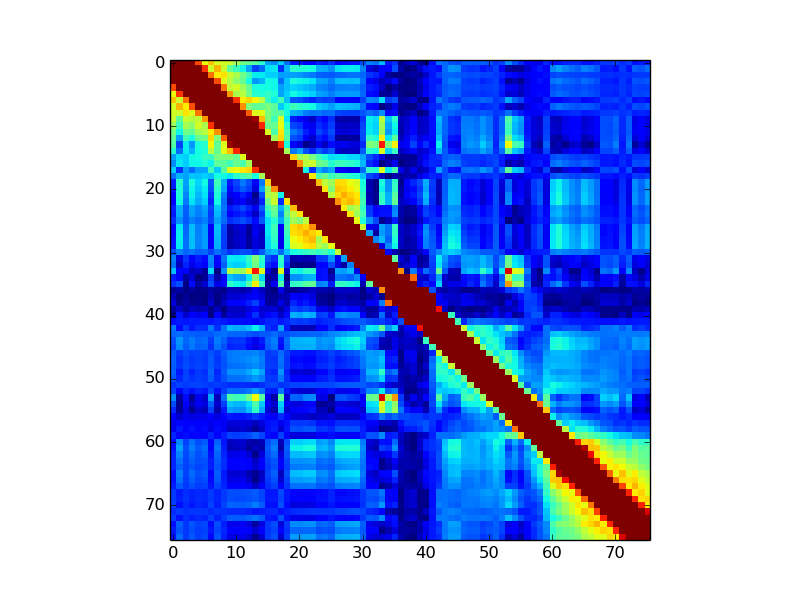
\includegraphics[height=0.5\textwidth]{images/fancy_figure.png}
    \caption{Awesome Image}
    \label{fig:awesome_image}
  \end{figure}

\end{document}
